\section {Molecular Orientation}

Understanding the orientation of succinic acid molecules helps us understand the chemistry taking place, and to interpret our experimental results. To build a clearer image of how succinic acid orients throughout the water interface, we have calculated bivariate angular distributions to define molecular orientation at various depths in the water surface. Figure \ref{fig:angle-definitions} depicts the succinic acid molecule and shows two angle definitions relative to the surface normal vector (labelled ``z'') that are used to define the molecular orientation. The angular tilt, $\theta$, is an angle between the O-C-O bisector axis of the carboxylic acid head group (pointing from the carbon to the oxygen end) and the vector normal to the plane of the water surface. $\theta$ varies from being aligned with the surface normal ($\theta=0$\textdegree), to perpendicular and in the plane of the surface ($\theta=90$\textdegree), to anti-aligned with the surface normal ($\theta=180$\textdegree) pointing in towards the water bulk. 

The carboxylic acid group twist angle, $\phi$, measures the angle between the plane formed by the O-C-O atoms of the carboxylic acid, and the plane formed by the O-C-O bisector and the surface normal vectors. This is a dihedral angle defined by the following three vectors: 1) the surface normal z-axis, 2) the O-C-O bisector axis, 3) and the C-O$_{carb}$ bond-vector of the acid group. Because of the symmetry of rotations about the carboxylic acid O-C-O bisector axis with respect to the plane of the water surface, $\phi$ has a range of 0\textdegree~$ \le \phi \le $180\textdegree. If $\phi=0$\textdegree~the plane of the O-C-O atoms is aligned perpendicularly to the water surface, and the C-O$_{carb}$ bond-vector points out of the surface away from the water bulk. Consequently, this same orientation causes the C-O$_{alc}$ bond to point towards the water bulk. A twist of $\phi=90$\textdegree~places both the O$_{carb}$ and O$_{alc}$ in the same plane, but parallel to the water surface (i.e. ``flat'' on the surface). $\phi=180$\textdegree~aligns the O-C-O plane similarly to $\phi=0$\textdegree, but with the C-O$_{alc}$ bond pointing out from the water surface, and the C-O$_{carb}$ pointing in towards the water bulk. 

\begin{figure}[h!]
	\begin{center}
		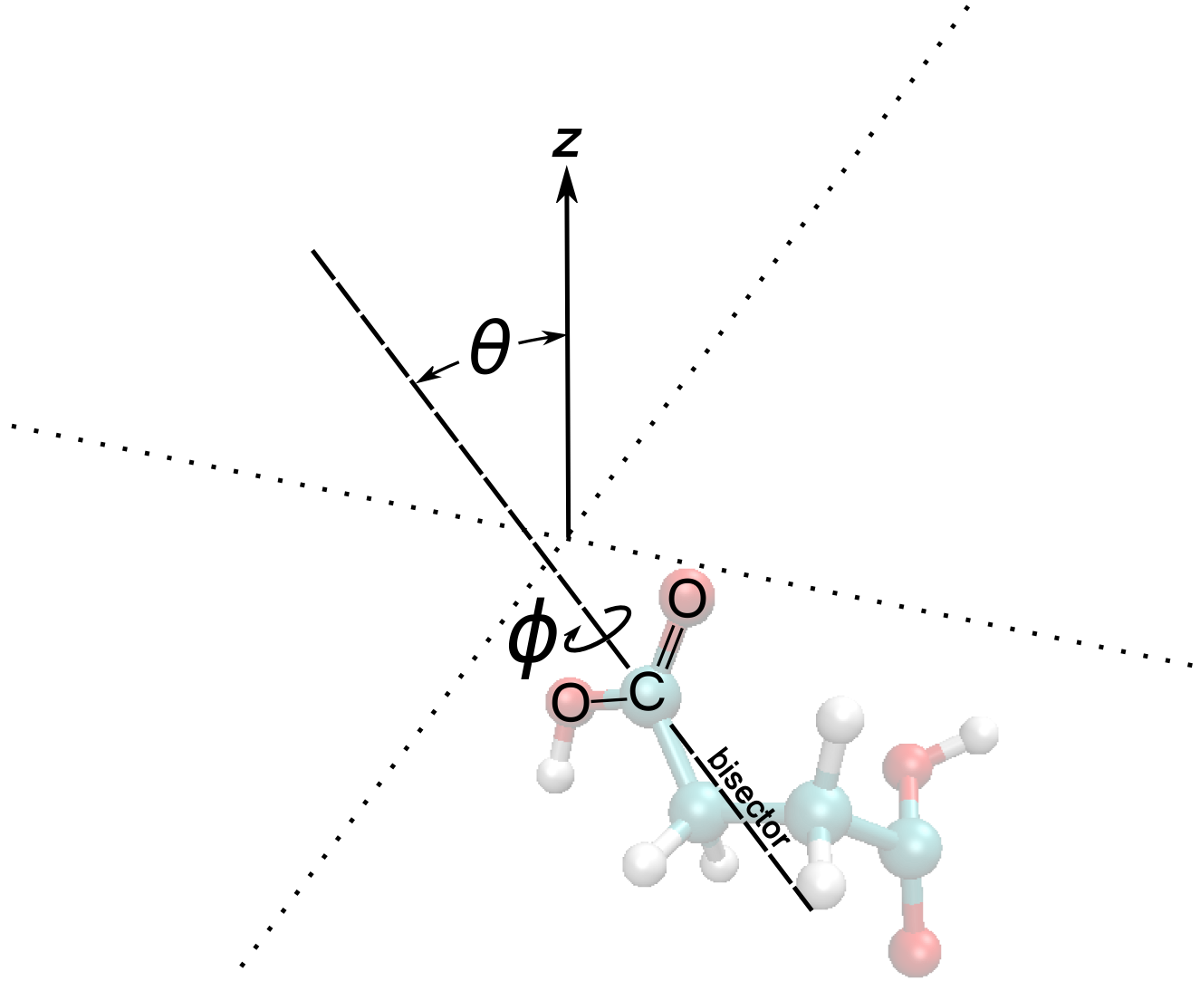
\includegraphics[scale=1.0]{images/bond-angles/bond-angle-definitions-small.png}
		\caption{Two angle definitions that characterize the carboxylic acid head group orientation relative to the water surface. The acid tilt, $\theta$, measures an angle formed between the O-C-O bisector axis of the acid group, and the vector normal to the plane of the water surface. Acid twist, $\phi$, is calculated as a dihedral formed by three vectors: the vector normal to the water surface, the O-C-O acid group bisector vector, and the C-O$_{carb}$ bond vector. This is equivalent to a rotation angle about the bisector axis, referenced to an orientation with the O-C-O plane perpendicular to the water surface. $\phi = 0$\textdegree~results from the carbonyl oxygen pointing further out towards the gas phase than the alcohol oxygen.}
		\label{fig:angle-definitions}
	\end{center}
\end{figure}

\subsection*{Dihedral}

A third angle, $\psi$, is the dihedral angle of the carbon backbone, where $\psi = 0$\textdegree~turns the succinic acid into a ``trans-'' carbon-chain configuration. Symmetry of rotations limits the range of dihedral twists to 0\textdegree~$\le \psi \le$ 180\textdegree.

Figure \ref{fig:dihedral} is an angular depth profile of the dihedral angle, $\psi$, on the y-axis, plotted against the distance of the molecular center of mass to the water surface, on the x-axis. Positions further into the water bulk appear on the left of the plot (negative values). The coloration ranges from dark blue to red, indicating low and high intensities of the 2D histogram, respectively. The greatest contribution is from the gauche configuration (60\textdegree) of the diacid. Clearly the molecule mostly has a $\psi$ value centered at 60\textdegree~at all depths, as indicated by the bright red streak running horizontally across the plot, centered at $\psi=60$\textdegree. There are minor contributions from the cis-configuration of the carbon backbone at $\psi = 180$\textdegree. The $180$\textdegree~configuration is represented throughout the deeper regions of the interface and in the water bulk. Near -2\angs~and further towards the surface near 0\angs, the distribution completely shifts to the $60$\textdegree~gauche configuration.


\begin{figure}[h!]
	\begin{center}
		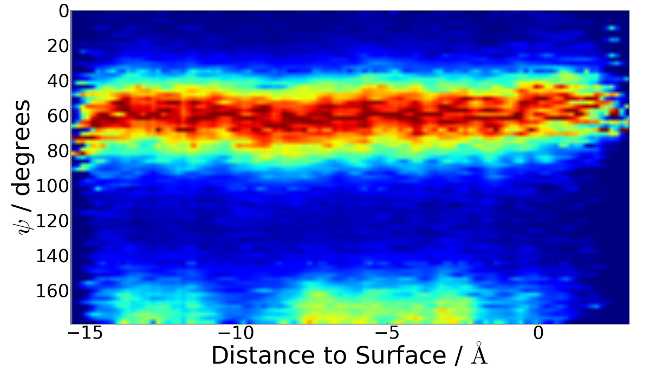
\includegraphics[scale=1.0]{images/dihedral/dihedral-small.png}
		\caption{The dihedral angle of the carbon backbone of the succinic acid molecule is found in either a gauche or cis- configuration. This angular depth profile shows the distribution of $\psi$ at different positions within the water interface. Dark blue and bright red coloration indicate low and high intensities of the histogram, respectively. The long streak of red centered at $\psi=60$\textdegree~shows the preference of the molecule to take on a gauche configuration throughout all depths from the water surface.}
		\label{fig:dihedral}
	\end{center}
\end{figure}


\subsection*{Carbonyl Group Orientation}

The acid group orientation distribution is depicted in Figure \ref{fig:carbonyl-theta-phi} at various depths throughout the interfacial water region. The plots each represent the bivariate $\theta$-$\phi$ distributions within a thin slice of the interface at a specific depth (labelled on each axis in the upper right). Negative positions are further into the water bulk, and positive depths are in the gas phase. The 0\angs~position is the water surface location as calculated through an averaging process of the positions of the outer-most waters of the slab. The areas of the distributions colored red are higher in intensity, and blue coloration denotes low intensity. Uniform coloration indicates isotropic orientational behavior of the two angles depicted.

Beginning at 2\angs~above the water surface, all those succinic acids that reside above the water surface location have a narrow orientational range in both $\theta$ and $\phi$. We see that the intensity in the topmost plot is centered around $\theta=135$\textdegree, and $\phi$ concentrates in the 0\textdegree-90\textdegree~range. This results from acid moieties that have their bisectors pointing mostly 45\textdegree~in towards the water bulk, and with the C-O$_{carb}$ directed either slightly out towards the gas phase (i.e. C-O$_{alc}$ points in towards the water bulk), or both C-O bonds align similarly with respect to the water surface. The intensity of this narrow orientational distribution increases at the 0\angs~depth, and the carboxylic oxygens remain pointing in towards the water bulk.

Moving just below the surface (-2\angs) we see the colored region shift to the center of the plot, indicating a carboxylic group that is both tilted parallel to the plane of the water surface, and also lying flat in the plane. This behavior is not altered at -4\angs, but the intensity of the orientational preference is reduced (i.e. there is less intense and more uniform coloration). At -6\angs and below into the water surface, the $\phi$ and $\theta$ distributions become increasingly isotropic.

The carbonyl groups have distinct behaviors throughout the interface, and can be grouped into three different orientations. At the interface and above ($\geq 0$\angs) the carboxylic acid O-C-O group points into the water surface (i.e. the bisector points towards the water bulk from the gas phase), and the carbonyl oxygen is either in the plane of the water surface, or pointing out towards the gas phase. Conversely, the alcohol oxygen is also in the plane of the surface, or pointing in towards the water bulk. Acid groups just below the surface (to depths of up to -4\angs) orient with the plane of the O-C-O atoms mostly parallel to the water surface. A depths further below in the water bulk the acid group loses orientational preference and the behavior is increasingly isotropic.

% Tilt/Twist
\begin{figure}[h!]
	\begin{center}
		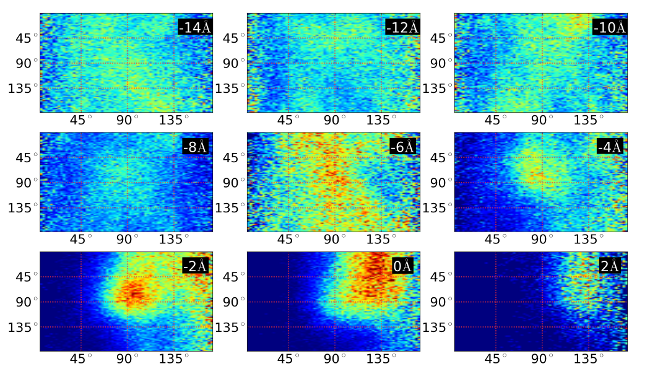
\includegraphics[scale=1.0]{images/bond-angles/carbonyl-theta-phi.png}
		\caption{The tilt and twist distributions of the carboxylic acid headgroups of the succinic acid ($\theta$ and $\phi$, respectively) characterize the orientation of the acid moiety relative to the water surface. Shown are several two-dimensional histograms of $\phi$ vs $\theta$ calculated at different depths of the interface (shown at the upper right of each axis). The depth value is calculated from the succinic acid molecular center of mass.} 
		\label{fig:carbonyl-theta-phi}
	\end{center}
\end{figure}


\subsection* {Methyl Group Orientation}

\begin{figure}[h!]
	\begin{center}
		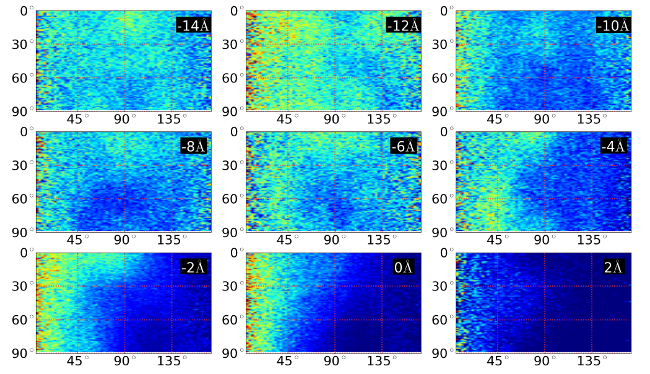
\includegraphics[scale=1.0]{images/bond-angles/methyl-theta-phi.png}
		\caption{Orientation of the diacid methyl groups is defined analogously to the carbonyl groups. The H-C-H atoms form a triatomic group for which both $\theta$ and $\phi$ are calculated. Shown here are the bivariate $\theta$-$\phi$ plots for various depths in the interfacial region of the aqueous slab. The plots are arranged similarly to those of Figure \ref{fig:carbonyl-theta-phi}. Because of the symmetry of the H-C-H, and the equivalence of the two hydrogens, the range of the twist is limited to 0\textdegree~$\leq \phi \leq$ 90\textdegree.}
		\label{fig:methyl-theta-phi}
	\end{center}
\end{figure}

The orientation of each methyl CH$_2$ group of the diacid is characterized using the same technique as was used for the O-C-O carbonyl groups. The definitions of $\theta$ and $\phi$ are analogously applied to the triatomic H-C-H groups for the analysis. The methyl group orientation distributions are plotted in Figure \ref{fig:methyl-theta-phi} for a range of depths through the water interface (arranged similarly to Figure \ref{fig:carbonyl-theta-phi}). The symmetry of the H-C-H group, and the equivalence of the two hydrogens, limits the range of $\phi$ to 0\textdegree~$\leq \phi \leq 90$\textdegree.

At all plotted depths down to -12\angs~there is intensity concentrated at $\theta=0$\textdegree. This concentration (i.e. orientational preference) is strongest near the water surface (-4\angs~- +2\angs). Just above the surface down to -2\angs~there is very little intensity for $\theta >90$\textdegree. This results from the methyl group bisector pointing mostly out of the water surface towards the gas phase, with the behavior strongest at or above 0\angs.

$\phi$ is necessarily isotropic for $\theta$ values near 0\textdegree. However, at -2\angs~and further out of the water phase, as $\theta$ increases the $\phi$ distribution becomes lopsided, and more intensity is found towards $\phi=0$\textdegree. Methyl groups with their bisectors tilting further towards the water surface are orienting perpendicularly to the plane of the surface. The -4\angs~plot shows the addition of intensity around $\phi=90$\textdegree~for $\theta \approx 90$\textdegree. These slightly deeper acids align the methyl groups both perpendicular and parallel to the plane of the surface. By -4\angs~and below, we see a much more isotropic distribution in $\phi$ at all values of $\theta$. However, the concentration around $\theta=0$\textdegree~remains, such that the methyl hydrogens points out of the water phase towards the gas.
